\documentclass[11pt, letterpaper]{article}
\usepackage[margin=1.5cm]{geometry}
\pagestyle{plain}

\usepackage{amsmath, amsfonts, amssymb, amsthm}
\usepackage{bbm}
\usepackage[shortlabels]{enumitem}
\usepackage[makeroom]{cancel}
\usepackage{graphicx}
\usepackage{xcolor}
\usepackage{array, booktabs, ragged2e}
\graphicspath{{./images/}}

\newcommand{\bs}[1]{\boldsymbol{#1}}
\newcommand{\mbb}[1]{\mathbb{#1}}
\newcommand{\mc}[1]{\mathcal{#1}}
\newcommand{\ra}[1]{\renewcommand{\arraystretch}{#1}}

\title{\bf Information Theory: Assignment I}
\author{\bf Connor Braun}
\date{}

\begin{document}
\maketitle
\noindent{\bf Problem 1} Let $X$ and $Y$ be discrete {\it r.v.}s with alphabets $\mc{X}=\{0,1\}$ and $\mc{Y}=\{0,1,2\}$ respectively,
with joint probability mass function $p_{XY}$ given by
\begin{align*}
    p_{XY}(0,0)&=P_{XY}(1,1)=\frac{1-\alpha}{2}\\
    p_{XY}(0,2)&=P_{XY}(1,2)=\frac{\alpha}{2}\\
    p_{XY}(0,1)&=P_{XY}(1,0)=0
\end{align*}
where $0<\alpha<1$. Determine (in bits) $H(X)$, $H(Y)$, $H(X|Y)$, $H(Y|X)$, $H(X,Y)$ and $I(X;Y)$ and depict these in a
Venn diagram.\\[10pt]
{\bf Solution} For this problem, all entropy quantities are in bits, as determine by the base two logarithms used in all computations.\\[10pt]
To begin we compute the marginal probability mass functions of $X$ and $Y$. These are very easy to determine from the joint probability mass function
and are given by
\begin{align*}
    p_Y(y)&=\sum_{x\in\mc{X}}p_{XY}(x,y)=\begin{cases}
        \frac{1-\alpha}{2},\quad\text{if $y=0$}\\
        \frac{1-\alpha}{2},\quad\text{if $y=1$}\\
        \alpha,\quad\text{if $y=2$}
    \end{cases}\\
    p_X(x)&=\sum_{y\in\mc{Y}}p_{XY}(x,y)=\begin{cases}
        \frac{1}{2},\quad\text{if $x=0$}\\
        \frac{1}{2},\quad\text{if $x=1$}.
    \end{cases}\\
\end{align*} 
Next we can use the marginal and joint probability mass functions to find $H(Y|X)$ directly.
\begin{align*}
    H(Y|X)&=-\sum_{x\in\mc{X}}\sum_{y\in\mc{Y}}p_{XY}(x,y)\log_2\frac{p_{XY}(x,y)}{p_X(x)}\\
    &=-\left(\frac{1-\alpha}{2}\log_2\left(\frac{1-\alpha}{2}\frac{2}{1}\right)+\frac{\alpha}{2}\log_2\left(\frac{\alpha}{2}\frac{2}{1}\right)+\frac{1-\alpha}{2}\log_2\left(\frac{1-\alpha}{2}\frac{2}{1}\right)+\frac{\alpha}{2}\log_2\left(\frac{\alpha}{2}\frac{2}{1}\right)\right)\\
    &=-\left((1-\alpha)\log_2(1-\alpha)+\alpha\log_2(\alpha)\right)\\
    &=h_b(\alpha)
\end{align*}
where $h_b(\alpha)$ is the binary entropy function. We proceed to compute the marginal entropies $H(X)$ and $H(Y)$ directly.
\begin{align*}
    H(X)&=-\sum_{x\in\mc{X}}p_X(x)\log_2p_X(x)\\
    &=-\left(\frac{1}{2}\log_2\frac{1}{2}+\frac{1}{2}\log_2\frac{1}{2}\right)\\
    &=1\\
    H(Y)&=-\sum_{y\in\mc{Y}}p_Y(y)\log_2p_Y(y)\\
    &=-\left(\frac{1-\alpha}{2}\log_2\frac{1-\alpha}{2}+\frac{1-\alpha}{2}\log_2\frac{1-\alpha}{2}+\alpha\log_2\alpha\right)\\
    &=-\left((1-\alpha)\log_2\frac{1-\alpha}{2}+\alpha\log_2\alpha\right).
\end{align*}
Equipped with these, we can compute the joint entropy $H(X,Y)$ and conditional entropy $H(X|Y)$ from the chain rule
\begin{align*}
    H(X,Y)&=H(X)+H(Y|X)\\
    &=1+h_b(\alpha)\\
    H(X|Y)&=H(X)+H(Y|X)-H(Y)\\
    &=1+h_b(\alpha)+(1-\alpha)\log_2\frac{1-\alpha}{2}+\alpha\log_2\alpha\\
    &=1-(1-\alpha)\log_2(1-\alpha)-\alpha\log_2\alpha+(1-\alpha)\log_2\frac{1-\alpha}{2}+\alpha\log_2\alpha\\
    &=1+(1-\alpha)\log_2\left(\frac{1-\alpha}{2}\frac{1}{1-\alpha}\right)\\
    &=1-(1-\alpha)\log_22\\
    &=\alpha
\end{align*}
and finally, using the definition of mutual information, we get $I(X;Y)=H(X)-H(X|Y)=1-\alpha$. The relationships between these measures can be compactly depicted
as a Venn diagram.
\begin{center}
  \makebox[\textwidth]{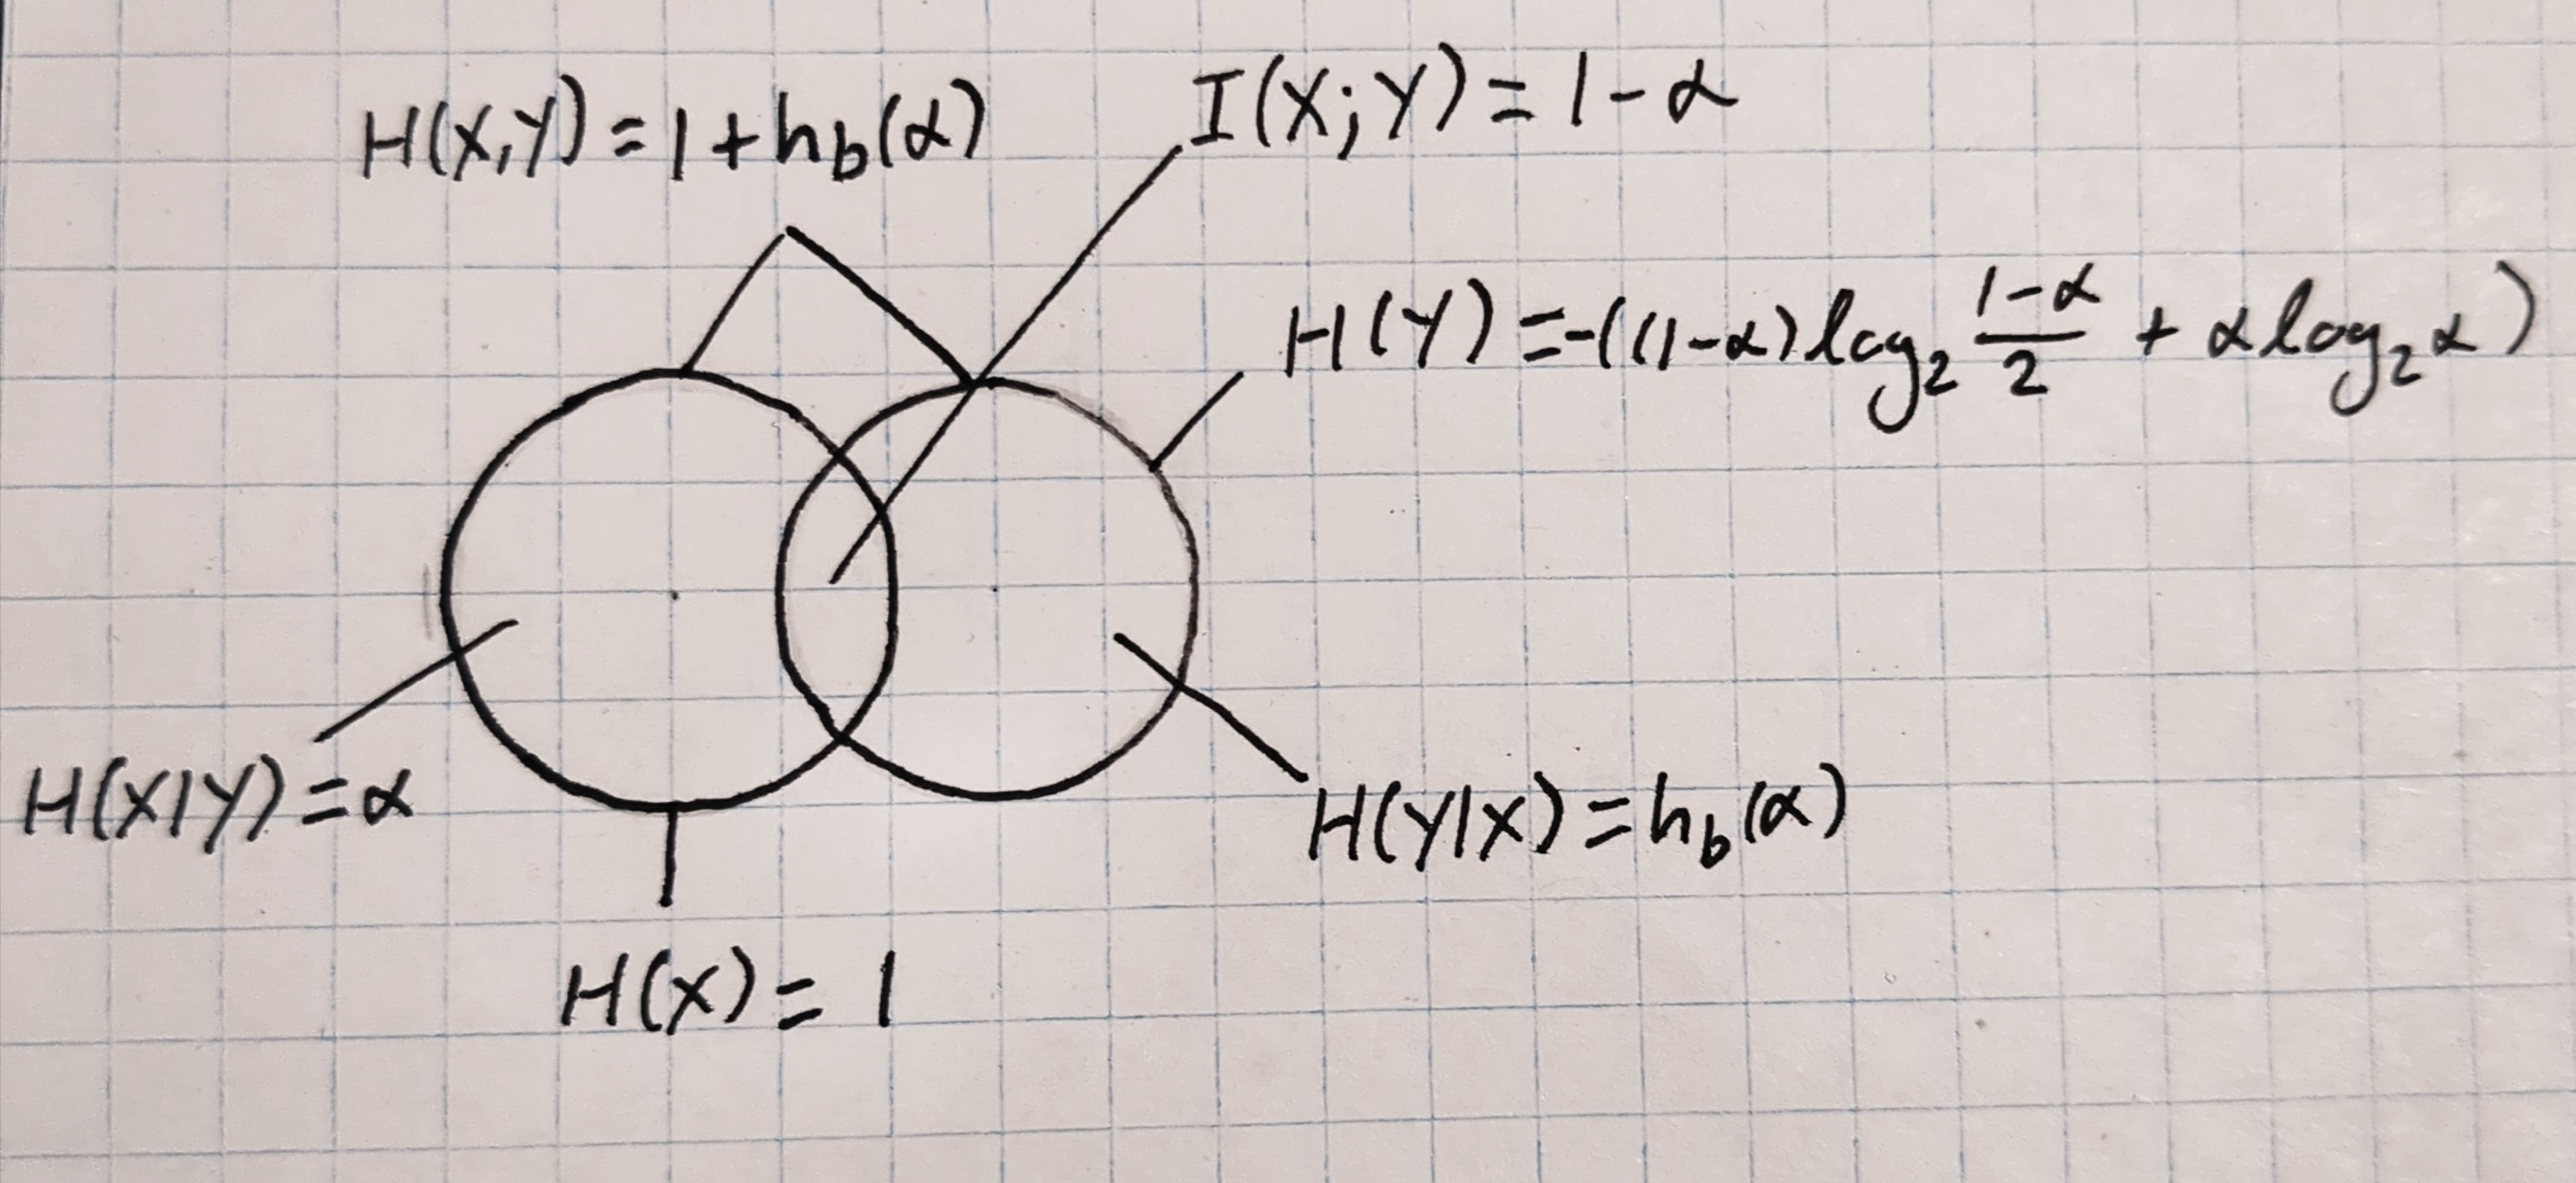
\includegraphics[width=130mm]{entropy-venn.jpg}}
\end{center}
{\bf Figure 1} Venn diagram depicting the relationships between the conditional, marginal and joint entropies of discrete {\it r.v.}s $X$ and $Y$, along with
the mutual information between $X$ and $Y$, denoted $I(X;Y)$.\\[10pt]

\noindent{\bf Problem 2} For each experiment described below involving random variables $X$ and $Y$, determine $I(X;Y)$ in bits.\\[10pt]
{\bf a)} You toss a biased coin with probability of heads given by $p$, with $0<p\leq 1/2$. Let $X$ be the event the coin comes up heads, and $Y$
the event it comes up tails.\\[10pt]
{\bf Solution} Noting that $X\sim Bernoulli(p)$ and $Y\sim Bernoulli(1-p)$ (i.e., $X=1$ for heads, $X=0$ for tails, $Y=1$ for tails and $Y=0$ for heads), we have $H(X)=h_b(p)$ and $H(Y)=h_b(1-p)$, where $h_b(\cdot)$ is the binary
entropy function, accepting arguments in the interval $[0,1]$. But these two entropies are equal for any fixed $p\in[0,1]$, since
\[h_b(p)=-p\log_2p-(1-p)\log_2(1-p)=-(1-p)\log_2(1-p)-p\log_2p=h_b(1-p)\]
so now $H(X)=H(Y)$. Since $\{X=j\}\cap\{Y=j\}=\emptyset$ for $j=0,1$ (i.e., $X$ and $Y$ are mutually exclusive) their joint probability mass function is given by
\begin{align*}
    p_{XY}(x,y)=\begin{cases}
        p,\quad\text{if $(x,y)=(1,0)$}\\
        0,\quad\text{if $(x,y)=(0,0)$}\\
        0,\quad\text{if $(x,y)=(1,1)$}\\
        1-p,\quad\text{if $(x,y)=(0,1)$}
    \end{cases}
\end{align*}
which enables us to compute the conditional entropy $H(X|Y)$ directly from the definition
\begin{align*}
    H(X|Y)&=-\sum_{y\in\{0,1\}}\sum_{x\in\{0,1\}}p_{XY}(x,y)\log_2\frac{p_{XY}(x,y)}{p_Y(y)}\\
    &=-\left(p\log_2\frac{p}{p}+(1-p)\log_2\frac{1-p}{1-p}\right)\\
    &=0.
\end{align*}
That is, there is no uncertainty in the outcome of $X$ if $Y$ is known -- a sensible conclusion, since we're flipping a coin, so the face-down side is determined by the face-up side. The mutual information between $X$ and $Y$
is then computed by the difference between the marginal and conditional entropies
\[I(X;Y)=H(X)-H(X|Y)=h_b(p)-0=h_b(p)\]
which is just the binary entropy function evaluated at $p$.\\[10pt]
{\bf b)} You roll a fair die. Here $X$ denotes the top side of the die, and $Y$ denotes the front side.\\[10pt]
{\bf Solution} Let $D_6=\{1,2,3,4,5,6\}$ be the set of faces of our die, and notice that $X\sim discrete\;uniform(1,6)$ and $Y\sim discrete\;uniform(1,6)$, so that
\[p_X(x)=\frac{1}{6},\quad\text{and}\quad p_Y(y)=\frac{1}{6}\]
$\forall x,y\in D_6$. Upon rolling the die, one side is face up, and another is face down, so neither can be on the front side. The remaining four sides can still be, however, and
the probability that any one of these sides is front-facing is uniformly distributed, since $Y$ is. Thus, for any $x\in D_6$, let $i_j^x$ for $j=1,2,3,4$ be the four faces which share an edge with
$x$ on our cubic die. Denote $D_6^x=\{i^x_1,i^x_2,i^x_3,i^x_4\}$. Then the conditional probability mass function of $Y|X$ is
\begin{align*}
    p_{Y|X}(y|x)=\begin{cases}
        \frac{1}{4},\quad\text{if $y\in D_6^x$}\\
        0,\quad\text{if $y\in D_6\setminus D_6^x$}.
    \end{cases}
\end{align*}
Since both the marginal and conditional distributions are uniformly distributed on their support, we have
\[H(X)=H(Y)=\log_2|D_6|,\quad\text{and}\quad H(Y|X=x)=\log_2|D_6^x|\tag{Lemma 2.6}\]
so that the mutual information can be computed from the definition
\[I(X;Y)=I(Y;X)=H(Y)-H(Y|X=x)=\log_2|D_6|-\log_2|D_6^x|=\log_26-\log_24=\log_2\frac{3}{2}\]
and we are done.\\[10pt]
{\bf Problem 3} Let $X$ and $Y$ be two jointly distributed discrete {\it r.v.}s with identical marginal distributions.
Define $\beta(X,Y)$ as
\[\beta(X,Y)=1-\frac{H(Y|X)}{H(X)}.\]
{\bf a)} Compare $\beta(X,Y)$ to $\frac{I(X;Y)}{H(X)}$.\\[10pt]
{\bf Solution} Exploring the relationship between $\beta(X,Y)$ and $\frac{I(X;Y)}{H(X)}$, we find
\begin{align*}
    \frac{I(X;Y)}{H(X)}&=\frac{H(X)+H(Y)-H(X,Y)}{H(X)}\\
    &=1+\frac{H(Y)-H(X)-H(Y|X)}{H(X)}\tag{expanding $H(X,Y)=H(X)+H(Y|X)$}\\
    &=1-\frac{H(Y|X)}{H(X)}+\frac{H(Y)-H(X)}{H(X)}\\
    &=\beta(X,Y)+\frac{H(Y)-H(X)}{H(X)}.\tag{1}
\end{align*}
From this, we glean the following relationship
\begin{align*}
    \begin{cases}
        \frac{I(X;Y)}{H(X)}<\beta(X,Y),\quad\text{if $H(X)>H(Y)$}\\[5pt]
        \frac{I(X;Y)}{H(X)}>\beta(X,Y),\quad\text{if $H(X)<H(Y)$}\\[5pt]
        \frac{I(X;Y)}{H(X)}=\beta(X,Y),\quad\text{if $H(X)=H(Y)$}
    \end{cases}\tag{2}
\end{align*}
which follows from (1) since $H(W)\geq 0$ for any {\it r.v.} $W$ (with equality iff $W$ is deterministic).\\[10pt]
{\bf b)} Is $\beta(X,Y)=\beta(Y,X)$?\\[10pt]
{\bf Solution} Not in general, since we have
\begin{align*}
    \beta(X,Y)&=\frac{H(X)-H(Y|X)}{H(X)}\\
    &=\frac{H(X)-H(Y)+I(X;Y)}{H(X)}\tag{since $H(Y|X)=H(Y)-I(X;Y)$}\\
    &=\frac{I(X;Y)}{H(X)}+\frac{H(X)-H(Y)}{H(X)}\\
    &\neq\frac{I(X;Y)}{H(Y)}+\frac{H(Y)-H(X)}{H(Y)}\tag{3}\\
    &=\frac{H(Y)}{H(Y)}+\frac{-H(X)+I(X,Y)}{H(Y)}\\
    &=1-\frac{H(X|Y)}{H(Y)}\\
    &=\beta(Y,X)
\end{align*}
where we instead have equality in (3) iff $H(X)=H(Y)$. Thus, $\beta(X,Y)=\beta(Y,X)$ iff $H(X)=H(Y)$. It should be noted that, while we continue to analyze the general case,
the distributions (that is, the probability mass function and support) of $X$ and $Y$ are identical, so we in fact have $H(X)=H(Y)$ and further $\beta(X,Y)=\beta(Y,X)$ in this problem.\\[10pt]
{\bf c)} Show that $0\leq \beta(X,Y)\leq 1$.\\[10pt]
{\bf Proof} First note that
\[\frac{I(X;Y)}{H(X)}=\frac{H(X)-H(X|Y)}{H(X)}\]
but $0\leq H(X|Y)\leq H(X)$, with $H(X|Y)=0$ iff $X|Y$ is deterministic and $H(X|Y)=H(X)$ iff $X$ and $Y$ are independent.
From this, we get
\[0=\frac{H(X)-H(X)}{H(X)}\leq\frac{H(X)-H(Y|X)}{H(X)}\leq\frac{H(X)-0}{H(X)}=1\]
so that $0\leq I(X;Y)/H(X)\leq 1$. Referring back to (2) in part {\bf a)}, we now have 
\[\beta(X,Y)\leq \frac{I(X;Y)}{H(X)}\leq 1\]
provided $H(X)\leq H(Y)$. Thus, we need only find an upper bound on $\beta(X,Y)$ in the case $H(X)>H(Y)$. To refine this objective, and
simultaneously establish a lower bound on $\beta(X,Y)$, consider the following:
\begin{align*}
    0\leq\beta(X,Y)\leq 1&\Leftrightarrow 0\leq 1-\frac{H(Y|X)}{H(X)}\leq 1\\
    &\Leftrightarrow -1\leq -\frac{H(Y|X)}{H(X)}\leq 0\\
    &\Leftrightarrow 0\leq\frac{H(Y|X)}{H(X)}\leq 1\\
    &\Leftrightarrow 0\leq H(Y|X)\leq H(X).\tag{4}
\end{align*}
Thus, showing that $0\leq H(Y|X)\leq H(X)$ gives us $0\leq\beta(X,Y)\leq 1$.\\[10pt]
We already know that $H(Y|X)\geq 0$, but show a brief proof for the sake of completeness. \\[10pt]
To see why $H(Y|X)\geq 0$, let $\mc{X}$ and $\mc{Y}$ be the alphabets of $X$ and $Y$ respectively, with joint probability mass function $p_{XY}(x,y)$ and
conditional probability mass function $p_{Y|X}(y|x)$. Note that since $0\leq p_{Y|X}(y|x)\leq 1$, $\log_21/p_{X|Y}(x|y)\geq 0$. Therefore,
\[H(Y|X)=\sum_{x\in\mc{X}}\sum_{y\in\mc{Y}}p_{XY(x,y)\log_2\frac{1}{p_{Y|X}(y|x)}}\geq 0.\]
Returning to the right inequality in (4), we simply have
\begin{align*}
    H(Y|X)&\leq H(Y)\tag{since conditioning reduces entropy}\\
    &<H(X)\tag{5}
\end{align*}
where we are assuming (5) holds since, as previously discussed, when $H(X)\leq H(Y)$, we have $\beta(X,Y)\leq 1$. Thus when $H(X)>H(Y)$ we have $0\leq H(X|Y)\leq H(X)$ which gives us $0\leq \beta(X,Y)\leq 1$, 
and otherwise we have $0\leq\beta(X,Y)\leq I(X;Y)/H(X)\leq 1$. So, in all cases, $0\leq \beta(X,Y)\leq 1$.\hfill{$\qed$}\\[10pt]
{\bf d)} When is $\beta(X,Y)=0$?\\[10pt]
{\bf Solution} Setting $\beta(X,Y)=0$, we find that
\[\beta(X,Y)=0\Rightarrow 1-\frac{H(Y|X)}{H(X)}=0\Rightarrow\frac{H(Y|X)}{H(X)}=1\Rightarrow H(Y|X)=H(X).\]
which occurs when $X$ and $Y$ are independent and have the same entropy, since then $H(Y|X)=H(Y)=H(X)$. Note once more that in this problem, the distributions of $X$ and $Y$ are identical, so we have $H(X)=H(Y)$.\\[10pt]
{\bf e)} Under what conditions is $\beta(X,Y)=1$?\\[10pt]
{\bf Solution} Setting $\beta(X,Y)=1$, we find that
\[\beta(X,Y)=1\Rightarrow 1-\frac{H(Y|X)}{H(X)}=1\Rightarrow\frac{H(Y|X)}{H(X)}=0\]
which occurs when $H(Y|X)=0$. This could mean that either $Y$ is deterministic, or $Y$ is deterministic given $X$. Since $X$ and $Y$ have identical distributions in this problem, $Y$ deterministic implies that $X$ is too, which
would produce $H(X)=0$ in the denominator, and render $\beta(X,Y)$ undefined. Thus, assuming neither $X$, $Y$ deterministic marginally, we require $H(Y|X)=0$, or equivalently $I(Y;X)=H(Y)$.\\[10pt]
{\bf Problem 4} Prove or disprove each of the following statements.\\[10pt]
{\bf a)} Let $X$ and $Y$ be independent discrete {\it r.v.}s. Then $H(X+Y)\geq\max\{H(X),H(Y)\}$.\\[10pt]
{\bf Solution} The statement is true.\\[10pt]
{\bf Proof} Let $\mc{X}$ and $\mc{Y}$ be the alphabets of $X$ and $Y$ respectively, with probability mass functions $p_X(x)$ and $p_Y(y)$ for $x\in\mc{X}$ and $y\in\mc{Y}$.
We will show that both $H(X+Y)\geq H(X)$ and $H(X+Y)\geq H(Y)$. Each inequality is obtained by precisely the same argument, but we will show both
for completeness.
\begin{align*}
    H(X+Y)&=H(Y)-H(Y|X+Y)+H(X+Y|Y)\\
    &=H(Y)-H(Y|X+Y)+H(X)\tag{6}\\
    &=H(X)+I(Y;X+Y)\\
    &\geq H(X)
\end{align*}
where the inequality above holds since $I(Y;X+Y)\geq 0$, with equality iff $Y$ and $X+Y$ are independent. To justify (6), we note that
\[Pr(X+Y=x+y|Y=y)=Pr(X+y=x+y|Y=y)=Pr(X=x|Y=y)=Pr(X=x)\]
where the last equality holds since $X$ is indpenendent of $Y$. Letting $p_{X+Y|Y}(x+y|y)$ be the conditional probability mass functions of $X+Y|Y$,
the above says that $p_{X+Y|Y}(x+y|y)=p_X(x)$ so
\begin{align*}
    H(X+Y|Y)&=-\sum_{x\in\mc{X}}\sum_{y\in\mc{Y}}p_Y(y)p_{X+Y|Y}(x+y|y)\log_2p_{X+Y|Y}(x+y|y)\\
    &=\sum_{y\in\mc{Y}}p_Y(y)\left(-\sum_{x\in\mc{X}}p_X(x)\log_2p_X(x)\right)\\
    &=H(X).
\end{align*}
To get $H(X+Y)\geq H(Y)$, the first argument is simply repeated.
\begin{align*}
    H(X+Y)&=H(X)-H(X|X+Y)+H(X+Y|X)\\
    &=H(X)-H(X|X+Y)+H(Y)\\
    &=H(Y)+I(X;X+Y)\\
    \geq H(Y).
\end{align*}
Since both $H(X+Y)\geq H(X)$ and $H(X+Y)\geq H(Y)$, $H(X+Y)\geq\max\{H(X),H(Y)\}$.\hfill{$\qed$}\\[10pt]
{\bf b)} Define the following two probability distributions on an alphabet of size $m$:
\[P=(p_1,p_2,p_3,\dots,p_m)\quad\text{and}\quad \tilde{P}=\left(\frac{p_1+p_2}{2},\frac{p_1+p_2}{2},p_3,\dots,p+m\right).\]
Then $H(P)>H(\tilde{P})$.\\[10pt]
{\bf Solution} The statement is false.\\[10pt]
{\bf Proof} We aim to prove the negation $H(\tilde{P})\geq H(P)\Leftrightarrow H(\tilde{P})-H(P)\geq 0$.
\begin{align*}
    H(\tilde{P})-H(P)&=\left(-2\frac{p_1+p_2}{2}\log_2\frac{p_1+p_2}{2}-p_3\log_2p_3-\dots-p_m\log_2p_m\right)+\left(p_1\log_2p_1+p_2\log_2p_2+\dots+p_m\log_2p_m\right)\\
    &=-(p_1+p_2)\log_2\frac{p_1+p_2}{2}+p_1\log_2p_1+p_2\log_2p_2\\
    &=p_1\log_2p_1-p_1\log_2\frac{p_1+p_2}{2}+p_2\log_2p_2-p_2\log_2\frac{p_1+p_2}{2}\\
    &=p_1\log_2\frac{2p_1}{p_1+p_2}+p_2\log_2\frac{2p_2}{p_1+p_2}\\
    &\geq \log_2e\left(p_1\left(1-\frac{p_1+p_2}{2p_1}\right)+p_2\left(1-\frac{p_1+p_2}{2p_2}\right)\right)\tag{fundamental inequality of the logarithm}\\
    &=\log_2e(p_1+p_2-p_1-p_2)\\
    &=0.
\end{align*}
So in fact we have $H(\tilde{P})-H(P)\geq 0\Rightarrow H(\tilde{P})\geq H(P)$.\hfill{$\qed$}\\[10pt]
{\bf c)} Let $X_1$, $X_2,\dots$ be {\it i.i.d.} with $X_1\sim Bernoulli(p=1/2)$. Let a success indicate an outcome of heads on a fair coin toss. Now let the random variable $L$
denote the number of tosses needed for the first head to appear. Then we have
\[I(L;X^L)=2.\tag{bits}\]
{\bf Solution} The statement is True.\\[10pt]
{\bf Proof} We first show a fact about the geometric series. For any $|x|<1$, we have
\[\sum_{n=0}^\infty x^n=\frac{1}{1-x}\quad\Rightarrow\quad \frac{d}{dx}\sum_{n=0}^\infty x^n=\frac{d}{dx}\frac{1}{1-x}\quad\Rightarrow\quad \sum_{n=0}^\infty nx^{n-1}=\frac{1}{(1-x)^2}.\]
Given this result, we can compute $H(L)$, since $L$ is a geometric random variable with success probability $p=1/2$. That is, its probability mass function $p_L$ is given by
\[p_L(k)=\left(\frac{1}{2}\right)^{k-1}\left(\frac{1}{2}\right)=\left(\frac{1}{2}\right)^k\]
for all $k\in\mbb{N}$. The entropy of $L$ is then
\begin{align*}
    H(L)&=-\sum_{k=1}^\infty \left(\frac{1}{2}\right)^k\log_2\left(\frac{1}{2}\right)^k\\
    &=\sum_{k=1}^\infty k\left(\frac{1}{2}\right)^k\\
    &=\frac{1}{2}\sum_{k=0}^\infty k\left(\frac{1}{2}\right)^{k-1}.
\end{align*}
Using the previously obtained fact about the geometric series, we get
\[H(L)=\frac{1}{2}\frac{1}{(1-1/2)^2}=\frac{4}{2}=2\]
so that the entropy of $L$ is 2 bits. Next, if we condition $L$ on the vector $X^L$, then $L$ is deterministic. That is, given a realized vector of tosses $X^L=(X_1,X_2,\dots,X_L)$,
where $X_j=1$ for at least one $j=1,2,\dots,L$, we have $L=\min\{j\in\{1,2,\dots,L\}: X_j=1\}$ with probability 1. This implies that $H(L|X^L)=0$, so finally the mutual information quantity of interest is determined to be
\[I(L;X^L)=H(L)-H(L|X^L)=2-0=2\]
as asserted.\hfill{$\qed$}\\[10pt]
{\bf Problem 5} Prove the following.\\[10pt]
{\bf a)} Given arbitrary $x_1,x_2,\dots x_n$, we have that
\[(x_1x_2\cdots x_n)^{1/n}\leq\frac{1}{n}\sum_{i=1}^nx_i.\]
{\bf Proof} We first note that $-\log x$ is convex on $(0,\infty)$ since
\[\frac{d^2}{dx^2}-\log x=\frac{1}{x^2}\geq 0\quad\forall x\in(0,\infty).\]
Further, we have that $\sum_{i=1}^n1/n=1$, and $x_i\in(0,\infty)$ for $i=1,2,\dots,n$, so
\begin{align*}
    -\log\left(\sum_{i=1}^n\frac{x_i}{n}\right)&\leq \sum_{i=1}^n-\frac{1}{n}\log x_i\tag{by convexity of $-\log x$ on $(0,\infty)$}\\
    &=-\sum_{i=1}^n\log x_i^{1/n}\\
    &=-\log\left(\prod_{i=1}^nx_i\right)^{1/n}
\end{align*}
which implies that
\begin{align*}
    \log\left(\prod_{i=1}^nx_i\right)^{1/n}&\leq\log\left(\sum_{i=1}^n\frac{x_i}{n}\right)\quad\Leftrightarrow (x_1x_2\cdots x_n)^{1/n}\leq\frac{1}{n}\sum_{i=1}^nx_i\tag{since $\log$ is monotonic increasing}
\end{align*}
and we are done.\hfill{$\qed$}\\[10pt]
{\bf b)} Consider two distributions $P_1$ and $P_2$ defined on a common alphabet $\mc{X}$ (where both $P_1(a)$,$P_2(s)>0$ $\forall x\in\mc{X}$).
Let $M:=1/2P_1+1/2P_2$ be a mixture distribution. Then
\[D(P_1\|P_2)\geq 2D(P_1\|M).\]
{\bf Proof} This result follows from the convexity of the Kullback-Leibler divergence in both of its arguments. That is,
\begin{align*}
    D(P_1\|M)&=D(1/2P_1+1/2P_1\|1/2P_1+1/2P_2)\\
    &\leq \frac{1}{2}D(P_1\|P_2)+\frac{1}{2}D(P_1\|P_1)\\
    &=\frac{1}{2}D(P_1\|P_2)\tag{since $D(P_1\|P_1)=0$}\\
    \Rightarrow\quad 2D(P_1\|M)&\leq D(P_1\|P_2)
\end{align*}
and we are done.\hfill{$\qed$}\\[10pt]
{\bf c) (2.28)} Let $X$ and $Y$ be two jointly distributed random variables with finite respective alphabets $\mc{X}$ and $\mc{Y}$ and
joint probability mass function $P_{XY}$ defined on $\mc{X}\times\mc{Y}$. For any fixed $\varepsilon>0$, $Y$ is said to be $\varepsilon$-{\it independent}
from $X$ if
\[\sum_{x\in\mc{X}}P_X(x)\sum_{y\in\mc{Y}}|P_{Y|X}(y|x)-P_Y(y)|<\varepsilon,\tag{7}\]
where $P_X$ and $P_Y$ are the marginal probability mass functions of $X$ and $Y$ respectively and $P_{Y|X}$ is the conditional probability mass function
of $Y$ given $X$. If
\[I(X;Y)<\frac{\log_2(e)}{2}\varepsilon^2\]
then $Y$ is $\varepsilon$-independent from $X$.\\[10pt]
{\bf Proof} First note that (7) can be rewritten
\[\sum_{x\in\mc{X}}P_X(x)\sum_{y\in\mc{Y}}|P_{Y|X}(y|x)-P_Y(y)|=\sum_{x\in\mc{X}}P_X(x)\|P_{Y|X}-P_Y\|\]
where $\|P_{Y|X}-P_Y\|$ is the variational distance between the conditional distribtuion $P_{Y|X}$ and the marginal distribution $P_Y$. Modifying Pinsker's inequality (Lemma 2.37)
we get an upper bound for $\|P_{Y|X}-P_Y\|$.
\[\|P_{Y|X}-P_Y\|^2\cdot\frac{\log_2e}{2}\leq D(P_{Y|X}\|P_Y|P_X)\quad\Rightarrow\quad\|P_{Y|X}-P_Y\|\leq\left(\frac{2}{\log_2e}D(P_{Y|X}\|P_Y|P_X)\right)^{1/2}.\tag{8}\]
However, by expanding $D(P_{Y|X}\|P_Y|P_X)$ we find that
\begin{align*}
    D(P_{Y|X}\|P_Y|P_X)&=\sum_{x\in\mc{X}}P_X(x)\sum_{y\in\mc{Y}}P_{Y|X}(y|x)\log_2\frac{P_{Y|X}(y|x)}{P_Y(y)}\\
    &=\sum_{x\in\mc{X}}\sum_{y\in\mc{Y}}P_{Y|X}(y|x)P_X(x)\log_2\frac{P_{Y|X}(y|x)P_X(x)}{P_Y(y)P_X(x)}\\
    &=\sum_{x\in\mc{X}}\sum_{y\in\mc{Y}}P_{XY}(y,x)\log_2\frac{P_{XY}(y,x)}{P_Y(y)P_X(x)}\\
    &=D(P_{XY}\|P_YP_X)\\
    &=I(X;Y)
\end{align*}
which allows us to rewrite the variational distance upper bound in (8) as
\[\|P_{Y|X}-P_Y\|\leq\left(\frac{2}{\log_2e}I(X;Y)\right)^{1/2}.\]
Finally, fixing $\varepsilon>0$ and supposing that $I(X;Y)<\frac{\log_2e}{2}\varepsilon^2$, we have
\begin{align*}
    \sum_{x\in\mc{X}}P_X(x)\sum_{y\in\mc{Y}}|P_{Y|X}(y|x)-P_Y(y)|&=\sum_{x\in\mc{X}}P_X(x)\|P_{Y|X}-P_Y\|\\
    &\leq\sum_{x\in\mc{X}}P_X(x)\left(\frac{2}{\log_2e}I(X;Y)\right)^{1/2}\\
    &<\sum_{x\in\mc{X}}P_X(x)\left(\frac{2}{\log_2e}\frac{\log_2e}{2}\varepsilon^2\right)^{1/2}\\
    &=\sum_{x\in\mc{X}}P_X(x)\varepsilon\\
    &=\varepsilon
\end{align*}
which implies that $Y$ is $\varepsilon$-independent from $X$.\hfill{$\qed$}\\[10pt]
{\bf Problem 6} A study of {\it H\"older's inequality}.\\[10pt]
{\bf a)} Given two probability vectors $(p_1,p_2,\dots,p_m)$ and $(q_1,q_2,\dots,q_m)$ on the set $\{1,2,\cdots,m\}$, apply Jensen's inequality to
show that for $0<\lambda<1$
\[\sum_{i=1}^mq_i^\lambda p_i^{1-\lambda}\leq 1\]
and give a necessary and sufficient condition for equality.\\[10pt]
{\bf Solution} Let $X_i$ be a discrete {\it r.v.} with alphabet $\mc{X}_i=\{p_i,q_i\}$ and probabilities
$Pr(X_i=p_i)=\lambda$ and $Pr(X_i=q_i)=1-\lambda$ for $i=1,2,\dots m$. Now let $f(x)=\log(x)$, which is concave on
$(0,\infty)$. With these, Jensen's inequality says that
\[\mbb{E}_i[f(X_i)]\leq f(\mbb{E}_i[X_i])\]
with this, and fixing $1\leq i\leq m$, we have
\begin{align*}
    &\mbb{E}_i[f(X_i)]=\lambda\log p_i+(1-\lambda)\log q_i\leq f(\mbb{E}_i[X_i])=\log(\lambda p_i + (1-\lambda)q_i)\\
   \Rightarrow\qquad &\log(p_i^\lambda q_i^{1-\lambda})\leq\log(\lambda p_i+(1-\lambda)q_i)\tag{9}
\end{align*}
further, since $g(x)=e^x$ is strictly monotonically increasing on $\mbb{R}$, we can eliminate the logarithm to find
\begin{align*}
    &e^{\log(p_i^\lambda q_i^{1-\lambda})}\leq e^{\log(\lambda p_i+(1-\lambda)q_i)}\\
    \Rightarrow\qquad&p_i^\lambda q_i^{1-\lambda}\leq\lambda p_i+(1-\lambda)q_i.\tag{10}
\end{align*}
This inequality holds for any choice of $X_i$, so we can now sum over the indices $j=1,2,\dots,m$ to get the desired result.
\begin{align*}
    \sum_{j=1}^mp_j^\lambda q_j^{1-\lambda}&\leq\sum_{j=1}^m\lambda p_j+(1-\lambda)q_J\\
    &=\lambda\sum_{j=1}^mp_j+(1-\lambda)\sum_{j=1}^mq_j\\
    &=\lambda+1-\lambda\\
    &=1.
\end{align*}
To find a necessary and sufficient condition for equality, notice that each term in the sum $\sum_{j=1}^mp_j^\lambda q_j^{1-\lambda}$ is positive, so we
seek to maximize each of them individually. Further, each term is bounded by the inequality (10). To achieve equality in (10), we need equality in (9) since the exponential
function is strictly increasing.\\[10pt]
To find conditions for equality in (9), first notice that $f(x)=\log x$ is not only concave, but strictly so on $(0,\infty)$, since
\[\frac{d^2}{dx^2}f(x)=\frac{d}{dx}x^{-1}=-x^{-2}<0\qquad\forall x\in(0,\infty).\]
Thus, Jensen's inequality further furnishes equality in (9) iff $X_j=\mbb{E}_j[X_j]$ with probability 1 for $j=1,2,\dots,m$. However, from how the probability mass functions of
each of the $X_j$ were defined, this only occurs in one of two ways. First, when either $\lambda=1$ or $\lambda=0$, we get
\begin{align*}
    \lambda=1\quad\Rightarrow\quad\begin{cases}
        Pr(X_j=p_j)=1\\
        Pr(X_j=q_j)=0
    \end{cases}\quad\Rightarrow\mbb{E}_j[X_j]=p_j\quad\text{and}\quad\lambda=0\quad\Rightarrow\quad\begin{cases}
        Pr(X_j=p_j)=0\\
        Pr(X_j=q_j)=1
    \end{cases}\quad\Rightarrow\mbb{E}_j[X_j]=q_j
\end{align*}
for $j=1,2,\dots, m$ and with probability 1. Second, we can have $p_j=q_j$ so that $\mbb{E}_j[X_j]=\lambda p_j+(1-\lambda)q_j=p_j=q_j$ for $j=1,2,\dots m$.
Thus,
\[\sum_{j=1}^mp_j^\lambda q_j^{1-\lambda}=1\]
if and only if either $\lambda\in\{0,1\}$ or $p_j=q_j$ $\forall j$. In our specific problem where $\lambda\in(0,1)$, only the latter condition is possible.\hfill{$\qed$}\\[10pt]
{\bf b)} Given positive real numbers $a_i$ and $b_i$, $i=1,2,\dots,m$, show via an appropriate use of the bound in {\bf a)} that for any $0<\lambda<1$
\[\sum_{i=1}^ma_ib_i\leq\left(\sum_{i=1}^ma_i^{1/\lambda}\right)^{\lambda}\left(\sum_{i=1}^mb_i^{1/(1-\lambda)}\right)^{1-\lambda}\]
with equality iff for some contant $c$
\[a_i^{1/\lambda}=cb_i^{1/(1-\lambda)}\]
for all $i$.\\[10pt]
{\bf Proof} Define $\bs{a}=(a_1,a_2,\dots,a_m)$ and $\bs{b}=(b_1,b_2,\dots,b_m)$ and let $\lambda\in (0,1)$. Then, for $0<\gamma<1$, we define the function $\|\cdot\|_\gamma:\mbb{R}^m_{>0}\rightarrow\mbb{R}_{>0}$,
where for $\bs{x}=(x_1,x_2,\dots x_m)\in\mbb{R}^m_{>0}$, 
\[\|\bs{x}\|_\gamma=\left(\sum_{i=1}^mx_i^{1/\gamma}\right)^\gamma.\]
Next, define the probability vectors $\bs{p}=(p_1,p_2,\dots,p_m)\in\mbb{R}^m_{>0}$ and $\bs{q}=(q_1,q_2,\dots q_m)\in\mbb{R}^m_{>0}$ on the finite set $\{1,2,\dots, m\}$ by
\[p_i=\frac{a_i^{1/\lambda}}{\|\bs{a}\|_\lambda^{1/\lambda}}\quad\text{and}\quad q_i=\frac{b_i^{1/(1-\lambda)}}{\|\bs{b}\|_{1-\lambda}^{1/(1-\lambda)}}\]
for $i=1,2,\dots,m$. Notice that these vectors do indeed define a probability mass function on $\{1,2,\dots,m\}$, since
\[\sum_{i=1}^m\frac{a_i^{1/\lambda}}{\|\bs{a}\|_\lambda^{1/\lambda}}=\frac{\sum_{i=1}^ma_i^{1/\lambda}}{\sum_{i=1}^ma_i^{1/\lambda}}=1\quad\text{and}\quad\sum_{i=1}^m\frac{b_i^{1/(1-\lambda)}}{\|\bs{b}\|_{1-\lambda}^{1/(1-\lambda)}}=\frac{\sum_{i=1}^mb_i^{1/(1-\lambda)}}{\sum_{i=1}^mb_i^{1/(1-\lambda)}}=1.\]
Then, by the inequality discovered in part {\bf a)}, we have
\begin{align*}
    &\sum_{i=1}^mp_i^\lambda q_i^{1-\lambda}\leq 1\\
    \Rightarrow\quad&\sum_{i=1}^m\left(\frac{a_i^{1/\lambda}}{\|\bs{a}\|_\lambda^{1/\lambda}}\right)^\lambda\left(\frac{b_i^{1/(1-\lambda)}}{\|\bs{b}\|_{1-\lambda}^{1/(1-\lambda)}}\right)^{1-\lambda}\leq 1\\
    \Rightarrow\quad&\sum_{i=1}^m\frac{a_ib_i}{\|\bs{a}\|_\lambda\|\bs{b}\|_{1-\lambda}}\leq 1\\
    \Rightarrow\quad&\sum_{i=1}^ma_ib_i\leq\|\bs{a}\|_\lambda\|\bs{b}\|_{1-\lambda}\\
    \Rightarrow\quad&\sum_{i=1}^ma_ib_i\leq\left(\sum_{i=1}^ma_i^{1/\lambda}\right)^{\lambda}\left(\sum_{i=1}^mb_i^{1/(1-\lambda)}\right)^{1-\lambda}\tag{11}
\end{align*}
as desired. Since we are disallowed $\lambda\in\{0,1\}$, equality holds in (11) iff $p_i=q_i$ for $i=1,2,\dots m$. That is, we require
\[\frac{a_i^{1/\lambda}}{\|\bs{a}\|_\lambda^{1/\lambda}}=\frac{b_i^{1/(1-\lambda)}}{\|\bs{b}\|_{1-\lambda}^{1/(1-\lambda)}}\quad\Leftrightarrow\quad a_i^{1/\lambda}=\frac{\|\bs{a}\|_\lambda^{1/\lambda}}{\|\bs{b}\|_{1-\lambda}^{1/(1-\lambda)}}b_i^{1/(1-\lambda)}\]
for all $i$. Setting $c=\|\bs{a}\|_{\lambda}^{1/\lambda}/\|\bs{b}\|_{1-\lambda}^{1/(1-\lambda)}\in\mbb{R}$, we have the necessary and sufficient condition for equality in (11); that is that we require
\[a_i^{1/\lambda}=cb_i^{1/(1-\lambda)}\]
for all $i$.\hfill{$\qed$}\\[10pt]
{\bf c)} Another form of H\"older's inequality is as follows:
\[\sum_{i=1}^mp_ia_ib_i\leq\left(\sum_{i=1}^mp_ia_i^{1/\lambda}\right)^{\lambda}\left(\sum_{i=1}^mp_ib_i^{1/(1-\lambda)}\right)^{1-\lambda}\]
where $\bs{p}=(p_1,p_2,\dots,p_m)$ is a probability vector as in {\bf a)}. Prove this inequality, and show that equality holds iff
\[p_ia_i^{1/\lambda}=cp_ib_i^{1/(1-\lambda)}\]
for all $i$.\\[10pt]
{\bf Proof} The arguments are precisely those from part {\bf b)}. Let $\lambda\in(0,1)$ and define $\bs{a^p}=(p_1^\lambda a_1,p_2^\lambda a_2,\dots p_m^\lambda a_m)$ and $\bs{b^p}=(p_1^{1-\lambda}b_1,p_2^{1-\lambda}b_2,\dots,p_m^{1-\lambda}b_m)$.
For $0<\gamma<1$, define $\|\cdot\|_\gamma:\mbb{R}^m_{>0}\rightarrow\mbb{R}_{>0}$, where for $\bs{x}=(x_1,x_2,\dots,x_m)\in\mbb{R}^m_{>0}$
\[\|\bs{x}\|_\gamma=\left(\sum_{i=1}^mx_i^{1/\gamma}\right)^\gamma.\]
Next, define the probability vectors $\bs{r}=(r_1,r_2,\dots,r_m)\in\mbb{R}^m_{>0}$ and $\bs{s}=(s_1,s_2,\dots s_m)\in\mbb{R}^m_{>0}$ on the finite set $\{1,2,\dots, m\}$ by
\[r_i=\frac{p_ia_i^{1/\lambda}}{\|\bs{a^p}\|_\lambda^{1/\lambda}}\quad\text{and}\quad s_i=\frac{p_ib_i^{1/(1-\lambda)}}{\|\bs{b^p}\|_{1-\lambda}^{1/(1-\lambda)}}\]
for $i=1,2,\dots,m$. Notice that these vectors do indeed define a probability mass function on $\{1,2,\dots,m\}$, since
\[\sum_{i=1}^m\frac{p_ia_i^{1/\lambda}}{\|\bs{a^p}\|_\lambda^{1/\lambda}}=\frac{\sum_{i=1}^mp_ia_i^{1/\lambda}}{\sum_{i=1}^mp_ia_i^{1/\lambda}}=1\quad\text{and}\quad\sum_{i=1}^m\frac{p_ib_i^{1/(1-\lambda)}}{\|\bs{b^p}\|_{1-\lambda}^{1/(1-\lambda)}}=\frac{\sum_{i=1}^mp_ib_i^{1/(1-\lambda)}}{\sum_{i=1}^mp_ib_i^{1/(1-\lambda)}}=1.\]
Then, by the inequality discovered in part {\bf a)}, we have
\begin{align*}
    &\sum_{i=1}^mr_i^\lambda s_i^{1-\lambda}\leq 1\\
    \Rightarrow\quad&\sum_{i=1}^m\left(\frac{p_ia_i^{1/\lambda}}{\|\bs{a^p}\|_\lambda^{1/\lambda}}\right)^\lambda\left(\frac{p_ib_i^{1/(1-\lambda)}}{\|\bs{b^p}\|_{1-\lambda}^{1/(1-\lambda)}}\right)^{1-\lambda}\leq 1\\
    \Rightarrow\quad&\sum_{i=1}^m\frac{p_i^\lambda p_i^{1-\lambda}a_ib_i}{\|\bs{a^p}\|_\lambda\|\bs{b^p}\|_{1-\lambda}}\leq 1\\
    \Rightarrow\quad&\sum_{i=1}^mp_ia_ib_i\leq\|\bs{a^p}\|_\lambda\|\bs{b^p}\|_{1-\lambda}\\
    \Rightarrow\quad&\sum_{i=1}^mp_ia_ib_i\leq\left(\sum_{i=1}^mp_ia_i^{1/\lambda}\right)^{\lambda}\left(\sum_{i=1}^mp_ib_i^{1/(1-\lambda)}\right)^{1-\lambda}\tag{11}
\end{align*}
as desired. Since we are disallowed $\lambda\in\{0,1\}$, equality holds in (11) iff $r_i=s_i$ for $i=1,2,\dots m$. That is, we require
\[\frac{p_ia_i^{1/\lambda}}{\|\bs{a^p}\|_\lambda^{1/\lambda}}=\frac{p_ib_i^{1/(1-\lambda)}}{\|\bs{b^p}\|_{1-\lambda}^{1/(1-\lambda)}}\quad\Leftrightarrow\quad p_ia_i^{1/\lambda}=\frac{\|\bs{a^p}\|_\lambda^{1/\lambda}}{\|\bs{b^p}\|_{1-\lambda}^{1/(1-\lambda)}}p_ib_i^{1/(1-\lambda)}\]
for all $i$. Setting $c=\|\bs{a^p}\|_{\lambda}^{1/\lambda}/\|\bs{b^p}\|_{1-\lambda}^{1/(1-\lambda)}\in\mbb{R}$, we have the necessary and sufficient condition for equality in (11); that is that we require
\[p_ia_i^{1/\lambda}=cp_ib_i^{1/(1-\lambda)}\]
for all $i$.\hfill{$\qed$}\\[10pt]
\end{document}
